\documentclass[12pt]{article}
\usepackage[utf8]{inputenc}
\usepackage[T1]{fontenc}
\usepackage[spanish,es-lcroman]{babel}
\usepackage{amsmath}
\usepackage{amsthm}
\usepackage{amsfonts}
\usepackage{amssymb}
\usepackage{physics}
\usepackage{tikz}
\usepackage{float}
\usepackage{calc}
\usepackage[autostyle,spanish=mexican]{csquotes}
\usepackage[per-mode=symbol]{siunitx}
\usepackage{textcomp, gensymb}
\usepackage{multicol}
\usepackage{enumitem}
\usepackage{hyperref}
\usepackage{setspace}
\usepackage[left=2.00cm, right=2.00cm, top=2.00cm, 
     bottom=2.00cm]{geometry}
% \usepackage{Estilos/ColoresLatex}
\usepackage{makecell}
\usepackage{subcaption}
\usepackage[skip=10pt, indent=30pt]{parskip}
% \usepackage{scalerel}
\usepackage{scalerel}[2016-12-29]
\usepackage{biblatex}
\usepackage{cancel}
\usepackage{tcolorbox}
\usepackage{wrapfig}
\usepackage{multirow}

\definecolor{ao}{rgb}{0.0, 0.0, 1.0}

\hypersetup{
    colorlinks=true,
    linkcolor=ao,
    filecolor=magenta,      
    urlcolor=ao,
}

\newcommand{\ptilde}[1]{\ensuremath{{#1}^{\prime}}}
\newcommand{\stilde}[1]{\ensuremath{{#1}^{\prime \prime}}}
\newcommand{\ttilde}[1]{\ensuremath{{#1}^{\prime \prime \prime}}}
\newcommand{\ntilde}[2]{\ensuremath{{#1}^{(#2)}}}
\newcommand{\pderivada}[1]{\ensuremath{{#1}^{\prime}}}
\newcommand{\sderivada}[1]{\ensuremath{{#1}^{\prime \prime}}}
\newcommand{\tderivada}[1]{\ensuremath{{#1}^{\prime \prime \prime}}}
\newcommand{\nderivada}[2]{\ensuremath{{#1}^{(#2)}}}

\def\stretchint#1{\vcenter{\hbox{\stretchto[440]{\displaystyle\int}{#1}}}}
\def\scaleint#1{\vcenter{\hbox{\scaleto[3ex]{\displaystyle\int}{#1}}}}
\def\scaleiint#1{\vcenter{\hbox{\scaleto[6ex]{\displaystyle\iint}{#1}}}}
\def\scaleiiint#1{\vcenter{\hbox{\scaleto[6ex]{\displaystyle\iiint}{#1}}}}
\def\scaleoint#1{\vcenter{\hbox{\scaleto[3ex]{\displaystyle\oint}{#1}}}}
\def\bs{\mkern-12mu}

% \newcommand{\textbf}[2]{\textbf{\textcolor{#1}{#2}}}
\sisetup{per-mode=symbol}
\decimalpoint
\sisetup{bracket-numbers = false}
\newlength{\depthofsumsign}
\setlength{\depthofsumsign}{\depthof{$\sum$}}
\newcommand{\nsum}[1][1.4]{% only for \displaystyle
    \mathop{%
        \raisebox
            {-#1\depthofsumsign+1\depthofsumsign}
            {\scalebox
                {#1}
                {$\displaystyle\sum$}%
            }
    }
}

\AtBeginDocument{\RenewCommandCopy\qty\SI}
\ExplSyntaxOn
\msg_redirect_name:nnn { siunitx } { physics-pkg } { none }
\ExplSyntaxOff

\numberwithin{equation}{section}

\linespread{1.25}

\renewcommand{\labelenumii}{\theenumii}
\renewcommand{\theenumii}{\theenumi.\arabic{enumii}.}

\emergencystretch=1em

\title{\large{Esferas y la ecuación de Legendre}}
\date{}
\author{M. en C. Gustavo Contreras Mayén}

\begin{document}
\maketitle
\fontsize{14}{14}\selectfont
\spanishdecimal{.}
\tableofcontents
\newpage

\section{Ecuación de Laplace.}
\subsection{Coordenadas esféricas.}

Para resolver la ecuación de Laplace:
\begin{align*}
\laplacian{\Psi} = 0
\end{align*}
en un sistema coordenado esférico $(r, \theta, \varphi)$, hacemos el cambio entre el sistema cartesiano y el esférico. Teniendo entonces:
\begin{align}
\begin{aligned}[b]
\dfrac{1}{r^{2}} \pdv{r} \left( r^{2} \pdv{\Psi}{r} \right) &+ \dfrac{1}{r^{2} \, \sin \theta} \bigg[ \pdv{\theta} \left( \sin \theta \pdv{\Psi}{\theta} \right) + \\[0.5em]
&+ \dfrac{1}{\sin^{2} \theta} \, \pdv[2]{\Psi}{\varphi} \bigg] = 0
\end{aligned}
\label{eq:ecuacion_22_15}
\end{align}

\subsection{Separación de variables.}

Para ocupar la técnica de separación de variables, proponemos una solución del tipo:
\begin{align*}
\Psi (r, \theta, \varphi) = R (r) \, \Theta (\theta) \, \Phi (\varphi)
\end{align*}
Que sustituimos en la ec (\ref{eq:ecuacion_22_15}), y cuyo procedimiento ya sabemos realizar. Llegamos a:
\begin{align*}
\Theta \Phi \dfrac{1}{r^{2}} \, \dv{r} \left( r^{2} \dv{R}{r} \right) &+ \dfrac{R}{r^{2}} \bigg[ \dfrac{\Phi}{\sin \theta} \, \dv{\theta} \left( \sin \theta \dv{\Theta}{\theta} \right) + \\[0.5em]
&+ \dfrac{\Theta}{\sin^{2} \theta} \, \dv[2]{\Phi}{\varphi} \bigg] = 0
\end{align*}
donde cada derivada se realiza sobre cada una de las variables.

Al dividir entre $R \, \Theta \, \Phi$ y luego multiplicar por $r^{2}$, llegamos a:
\begin{align*}
\dfrac{1}{R} \, \dv{r} \left( r^{2} \dv{R}{r} \right) &+ \bigg[ \dfrac{1}{\Theta \sin \theta} \, \dv{\theta} \left( \sin \theta \dv{\Theta}{\theta} \right) + \\[0.5em]
&+ \dfrac{1}{\Phi \sin^{2} \theta} \, \dv[2]{\Phi}{\varphi} \bigg] = 0
\end{align*}
Ya que cada uno de los términos es función de variables independientes, por tanto deben de ser una constante, y las dos constantes deben de sumar cero. Así obtenemos:
\begin{align*}
\dfrac{1}{R} \, \dv{r} \left( r^{2} \dv{R}{r} \right) &= \alpha \\[0.5em]
\dfrac{1}{\Theta \sin \theta} \, \dv{\theta} \left( \sin \theta \dv{\Theta}{\theta} \right) + \dfrac{1}{\Phi \sin^{2} \theta} \, \dv[2]{\Phi}{\varphi} &= - \alpha
\end{align*}
La segunda ecuación debe de separarse nuevamente, agregamos $\alpha$ en ambos lados de la expresión y multiplicamos por $\sin^{2} \theta$, llegando a:
\begin{align*}
\dfrac{\sin \theta}{\Theta} \, \dv{\theta} &\left( \sin \theta \dv{\Theta}{\theta} \right) + \\[0.5em]
&+\alpha \, \sin^{2} \theta +  \dfrac{1}{\Phi} \, \dv[2]{\Psi}{\varphi} = 0
\end{align*}
Siguiendo el mismo razonamiento, tendremos una segunda constante de separación:
\begin{align*}
\dfrac{\sin \theta}{\Theta} \, \dv{\theta} \left( \sin \theta \dv{\Theta}{\theta} \right) &= \beta \\[0.5em]
\dfrac{1}{\Phi} \, \dv[2]{\Phi}{\varphi} = - \beta
\end{align*}
De modo que hemos recuperado tres EDO2H, cada una de una sola variable:
\begin{eqnarray}
\dfrac{1}{r^{2}} \, \dv{r} \left( r^{2} \dv{R}{r} \right) - \dfrac{\alpha}{r^{2}} \, R &=& 0 \label{eq:ecuacion_22_17a} \\[0.5em] 
\dfrac{1}{\sin \theta} \, \dv{\theta} \left( \sin \theta \dv{\Theta}{\theta} \right) + \left( \alpha - \dfrac{\beta}{\sin^{2} \theta} \right) \, \Theta &=& 0 \label{eq:ecuacion_22_17b} \\[0.5em] 
\dv[2]{\Phi}{\varphi} + \beta \, \Phi &=& 0 \label{eq:ecuacion_22_17c}
\end{eqnarray}
Identificamos las EDO:
\begin{enumerate}
\item La ec. (\ref{eq:ecuacion_22_17a}) se conoce como \textbf{ecuación radial}.
\item La ec. (\ref{eq:ecuacion_22_17b}) es la \textbf{ecuación polar}.
\item La tercera ec. (\ref{eq:ecuacion_22_17c}) es la \textbf{ecuación azimutal}.
\end{enumerate}

\subsection{Simetría azimutal.}

Consideramos el caso donde $\Phi$ es la función constante,  esto corresponde a problemas con una \textbf{simetría azimutal},  es decir, problemas para los cuales está claro \textbf{a priori} que el potencial es independiente del ángulo azimutal $\varphi$. En tales situaciones, la ec. \ref{eq:ecuacion_22_17c}) implica que $\beta = 0$ porque $\Phi$ es una constante (distinta de cero).
\par
Las variables independientes se reducen a dos: 
\begin{align*}
\psi (r, \theta) = R (r) \, \Theta (\theta)    
\end{align*}
Entonces se reduce a un sistema de dos EDO2H:
\begin{eqnarray}
\begin{aligned}
\dfrac{1}{r^{2}} \dv{r} \left( r^{2} \dv{R}{r} \right) - \dfrac{\alpha}{r^{2}} \, R &= 0 \\[0.5em]  
\dfrac{1}{\sin \theta} \dv{\theta} \left( \sin \theta \dv{\Theta}{\theta} \right) + \alpha \, \Theta &= 0
\end{aligned}
\label{eq:ecuacion_26_02}
\end{eqnarray}

\subsection{Resolviendo las EDO2H.}

De manera inicial nos enfocamos en la ecuación polar. La presencia en el denominador del término $\sin \theta \dd{\theta}$ (que es el diferencial de $\cos \theta)$ sugiere el cambio de variable de $\theta$ a $u \equiv \cos \theta$.
\par
Para cualquier función $f (\theta)$, con la regla de la cadena se tiene:
\begin{eqnarray*}
\begin{aligned}
\dv{f}{u} &= \dv{f}{\theta} \dv{\theta}{u} = \\[0.5em] 
&= \dv{f}{\theta} \dfrac{1}{\dv*{u}{\theta}} = \\[0.5em] 
&= - \dfrac{1}{\sin \theta} \dv{f}{\theta}
\end{aligned}
\end{eqnarray*}
De manera equivalente:
\begin{align}
\dv{f}{\theta} = - \sin \theta \dv{f}{u}
\label{eq:ecuacion_26_03}
\end{align}
Esto nos permite convertir la derivada de una función con respecto a $u$, en la derivada de la misma función con respecto a $\theta$.
\par
Proponemos una función $P(u)$ tal que:
\begin{align*}
P (u) = \Theta(\theta)
\end{align*}
Usamos la regla de la cadena mostrada, sustituyendo en la ecuación polar y escribiendo $\sin^{2} \theta = 1 - u^{2}$. La EDO pasa a ser:
\begin{align*}
- \dfrac{1}{\sin \theta} \dv{\theta} \bigg[ (1 - u^{2}) \dv{P}{u} \bigg] + \alpha \, P = 0
\end{align*}
El término en el corchete es función de $u$.
\par
Ocupando la ec. (\ref{eq:ecuacion_26_03}), podemos convertir la derivada en $\theta$ en una derivada en $u$, para así obtener:
\begin{align}
\dv{u} \bigg[ (1 - u^{2}) \dv{P}{u} \bigg] + \alpha P = 0
\label{eq:ecuacion_26_04}
\end{align}
Que se puede escribir como:
\begin{align}
(1 - u^{2}) \, \dv[2]{P}{u} - 2 \, u \, \dv{P}{u} + \alpha \, P = 0
\label{eq:ecuacion_26_05}
\end{align}
De manera equivalente:
\begin{align}
\dv[2]{P}{u} - \dfrac{2 \, u}{1 - u^{2}} \, \dv{P}{u} + \dfrac{\alpha}{(1 - u^{2})} \, P = 0
\label{eq:ecuacion_26_06}
\end{align}
A esta ecuación (\ref{eq:ecuacion_26_05}) - (\ref{eq:ecuacion_26_06}) se le conoce como la \textbf{ecuación diferencial de Legendre}.
\par
Las soluciones a la ecuación de Legendre son \textbf{los polinomios de Legendre de orden $n$}: $P_{n} (x)$, y se detallan en las notas de trabajo, por lo que aquí haremos uso de las mismas y de sus propiedades.

%Ref. Riley (2009) 18.1 Legendre functions.
\section{Funciones ordinarias de Legendre.}
\subsection{La ecuación diferencial.}

La ecuación diferencial ordinaria de Legendre tiene la forma:
\begin{align}
(1 - x^{2}) \sderivada{y} - 2 \, x \, \pderivada{y} + \ell (\ell + 1) \, y = 0
\label{eq:ecuacion_18_01}
\end{align}
y tiene tres puntos regulares singulares en $x = -1, 1, \infty$.
\par
Esta ecuación se presenta en diversos problemas de la física, en particular en problemas con simetría axial que involucra el operador $\nabla^{2}$, expresado en coordenadas esféricas. Normalmente la variable $x$ en la ecuación de Legendre es el coseno del ángulo en coordenadas polares, por lo que $-1 \leq x \leq 1$.
\par
El parámetro $\ell$ es un número real, y la solución a la ecuación (\ref{eq:ecuacion_18_01}) se le denomina \textbf{función ordinaria de Legendre}.
\par
Es posible demostrar que $x = 0$ es un punto ordinario, por lo que podemos esperar dos soluciones linealmente independientes de la forma:
\begin{align*}
y = \nsum_{n=0}^{\infty} a_{n} \, x^{n}
\end{align*}
Sustituimos entonces para encontrar:
\begin{align*}
&\nsum_{n=0}^{\infty} \bigg[ n \, (n - 1) a_{n} \, x^{n-2} - n \, (n - 1) \, a_{n} \, x^{n} + \\[0.5em]
&- 2 \, n \, a_{n} \, x^{n} + \ell (\ell + 1) \, a_{n} \, x^{n} \bigg] = 0
\end{align*}
Donde agrupamos los términos:
\begin{align*}
&\nsum_{n=0}^{\infty} \bigg[ (n + 2)(n + 1) \, a_{n+2} - [ n \, (n+1) + \\[0.5em]
&- \ell (\ell + 1) ] \, a_{n} \bigg] \, x^{n} = 0
\end{align*}
La relación de recurrencia es por tanto:
\begin{align}
a_{n+2} = \dfrac{[n \, (n + 1)- \ell (\ell + 1)]}{(n + 1)(n + 2)} \, a_{n}
\label{eq:ecuacion_18_02}
\end{align}
para $n = 0, 1, 2, \ldots$
Si elegimos $a_{0} = 1$ y $a_{1} = 0$ entonces obtenemos la solución:
\begin{align}
\begin{aligned}
y_{1} (x) &= 1 - \ell (\ell + 1) \dfrac{x^{2}}{2!} + \\
&+ (\ell - 2)\; \ell \; (\ell + 1)\;(\ell + 3) \dfrac{x^{4}}{4!} - \ldots
\end{aligned}
\label{eq:ecuacion_18_03}
\end{align}
Mientras que si escogemos $a_{0} = $ y $ a_{1} = 1 $, encontramos la segunda solución:
\begin{align}
\begin{aligned}
y_{2} (x) &= x - (\ell - 1)(\ell + 2) \dfrac{x^{3}}{3!} + \\[0.5em]
&+ (\ell - 3) (\ell - 1)(\ell + 2)(\ell + 4) \dfrac{x^{5}}{5!} - \ldots
\label{eq:ecuacion_18_04}
\end{aligned}
\end{align}
Aplicando la prueba de convergencia de la razón, se encuentra que ambas series convergen para $\abs{x} < 1$, y su radio de convergencia es unitario, que representa la distancia al punto singular más cercano de la ecuación.
\par
Dado que la ecuación (\ref{eq:ecuacion_18_03}) contiene sólo potencias pares de $x$ y la ecuación (\ref{eq:ecuacion_18_04}) contiene sólo potencias impares,  esas dos soluciones no pueden ser proporcionales una de la otra, por lo tanto, son linealmente independientes. De aquí, la solución general para la ecuación (\ref{eq:ecuacion_18_01}) y con $\abs{x} < 1$ es:
\begin{align*}
y (x) = c_{1} \, y_{1} (x) + c_{2} \, y_{2} (x)
\end{align*}

\subsection{Legendre para enteros \texorpdfstring{$\ell$}{l}.}

En varios problemas de la física, el parámetro $\ell$ en la ecuación de Legendre - ec. (\ref{eq:ecuacion_18_01})- es un entero, es decir $\ell = 0,1,2,\ldots$. En ese caso, la relación de recurrencia - ec. (\ref{eq:ecuacion_18_02})- queda como:
\begin{align*}
a_{\ell + 2} = \dfrac{[ \ell (\ell + 1) - \ell (\ell + 1) ]}{(\ell + 1)(\ell + 2)} \, a_{\ell} = 0
\end{align*}
Esto es, la serie termina y obtenemos una solución con un polinomio de orden $\ell$.
\par
En particular, si $\ell$ es par, entonces $y_{1} (x)$ en la ecuación (\ref{eq:ecuacion_18_03}) se reduce a un polinomio,  mientras que si $\ell$ es impar, lo mismo le ocurre a $y_{2} (x)$ en la ecuación (\ref{eq:ecuacion_18_04}).
\par
Esas soluciones (adecuadamente normalizadas) son llamadas \textbf{denim}{Polinomios ordinarios de Legendre de orden $\ell$}, se escriben $P_{\ell} (x)$ y son válidas para todo valor $x$ finito. De manera convencional, se normaliza $P_{\ell} (x)$ de tal manera que $P_{\ell}(1) =  1$, y como consecuencia $P_{\ell} (-1) = (-1)^{\ell}$.
\par
Los primeros polinomios se construyen fácilmente y están dados por:
\begin{center}
\begin{tabular}{l l}
$P_{0} (x) {=} 1 $ & $P_{1}(x) {=} 1 $ \\[0.5em]
$P_{2} (x) {=} \dfrac{1}{2} (3 x^{2} {-} 1)$ & $P_{3} (x) {=} \dfrac{1}{2} (5 x^{2} {-} 3 x)$ \\[0.5em] 
$P_{4} (x) {=} \dfrac{1}{8} (35 x^{4} {-} 30 x^{2} {+} 3)$ & $P_{5} (x) {=} \dfrac{1}{8} (63 x^{5} {-} 70 x^{3} + 15 x)$
\end{tabular}
\end{center}
Gráfica de los primeros polinomios de Legendre:
\begin{figure}[H]
    \centering
    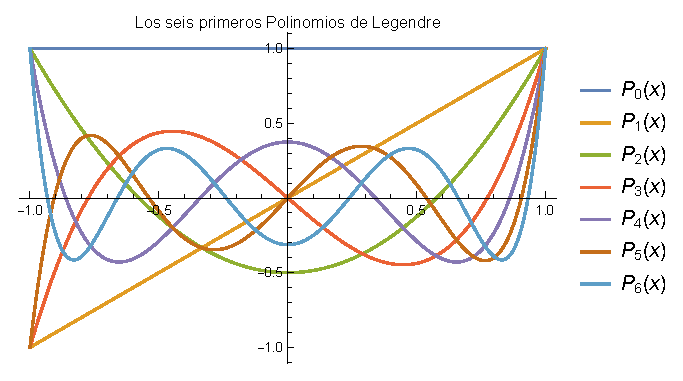
\includegraphics[scale=0.9]{Imagenes/Plot_Lagrange_0-6.eps}
    % \caption{Gráfica de los primeros seis polinomios de Legendre.}
    % \label{fig:polinomios_Lagrange_01}
\end{figure}
A pesar de que si $\ell$ es un entero par o impar, respectivamente para $y_{1}(x)$ - ec. (\ref{eq:ecuacion_18_03}) - o $y_{2}(x)$ - ec. (\ref{eq:ecuacion_18_04}),  se termina dando un múltiplo del correspondiente polinomio ordinario de Legendre $P_{\ell}(x)$,  la otra serie en cada caso no termina y por tanto converge sólo para $\abs{x} < 1$.
\par
Dependiendo de si $\ell$ es par o impar, se definen las \textbf{amethyst}{funciones ordinarias de Legendre de segunda clase} como:
\begin{align*}
Q_{\ell} (x) &=  \alpha_{\ell} \, y_{2} (x) \\
Q_{\ell} (x) &=  \beta_{\ell} \, y_{1} (x)
\end{align*}
respectivamente. Donde las constantes $\alpha_{\ell}$ y $\beta_{\ell}$ toman los valores:
\begin{align}
&\mbox{ para $\ell$ par} \nonumber \\
&\alpha_{\ell} = \dfrac{(-1)^{\ell/2} \; 2^{\ell} \; [(\ell / 2)!]^{2}}{\ell!} \label{eq:ecuacion_18_05} \\[1em]
&\mbox{ para $\ell$ impar} \nonumber \\
&\beta_{\ell} = \dfrac{(-1)^{(\ell + 1)/2} \; 2^{\ell - 1} \; \lbrace \left[ (\ell - 1) /2 \right] ! \rbrace^{2}}{\ell!} \label{eq:ecuacion_18_06}
\end{align}
La normalización de los factores se elige de tal manera que $Q_{\ell} (x)$ obedece la misma relación de recurrencia de $P_{\ell} (x)$.
\par
La solución general para la EDO de Legendre para enteros $\ell$ es por tanto:
\begin{align}
y (x) = c_{1} \, P_{\ell} (x) + c_{2} \, Q_{\ell} (x) 
\label{eq:ecuacion_18_07}
\end{align}
Donde $P_{\ell} (x)$ es un polinomio de orden $\ell$, que converge para cualquier $x$, y $Q_{\ell} (x)$ es una serie infinita que converge sólo si $\abs{x} < 1$.
\par
Usando el método del Wronkisano, podemos obtener una forma cerrada para $Q_{\ell} (x)$. Una segunda solución para la ecuación de Legendre (ec. \ref{eq:ecuacion_18_01}), con $\ell = 0$ es:
\begin{eqnarray}
\begin{aligned}[b]
y_{2} (x) &= P_{0} (x) \scaleint{6ex}^{x} \dfrac{1}{[P_{0} (u)]^{2}} \, \exp \left( \scaleint{6ex}^{u} \dfrac{2 \, v}{1 - v^{2}} \dd{v} \right) \dd{u} \\[0.5em] 
&= \scaleint{6ex}^{x} \exp [ - \ln (1 - u^{2}) ] \dd{u} \\[0.5em] 
&= \scaleint{6ex}^{x} \dfrac{\dd{u}}{(1 - u^{2})} = \dfrac{1}{2} \, \ln \left( \dfrac{1 + x}{1 - x} \right)
\end{aligned}
\label{eq:ecuacion_18_08}
\end{eqnarray}
En la segunda línea hemos utilizado el hecho de que $P_{0} (x) = 1$.
\par
Lo que queda es ajustar la normalización de esta solución para que se corresponda con la ecuación (\ref{eq:ecuacion_18_05}). Expandiendo el logaritmo en la ec. (\ref{eq:ecuacion_18_08}) como una serie de Maclaurin, obtenemos:
\begin{align*}
y_{2} (x) = x + \dfrac{x^{3}}{3} + \dfrac{x^{5}}{5} + \cdots
\end{align*}
Gráfica de la segunda solución:
\begin{figure}[H]
    \centering
    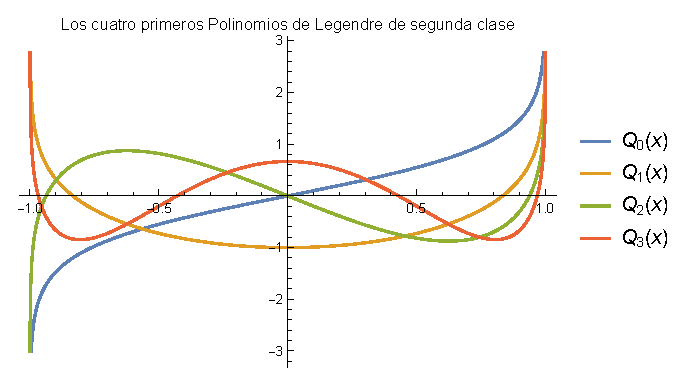
\includegraphics[scale=0.9]{Imagenes/Plot_LagrangeSC_0-4.eps}
    % \caption{Gráfica de los cuatro polinomios de Legendre de segunda clase.}
    % \label{fig:polinomios_Lagrange_02}
\end{figure}
Comparando esto con la expresión para $Q_{0} (x)$, usando la ec. (\ref{eq:ecuacion_18_04}) con $\ell = 0$ y normalizando -ec. (\ref{eq:ecuacion_18_05})-, encontramos que $y_{2} (x)$ está correctamente normalizada, así:
\begin{align*}
Q_{0} (x) = \dfrac{1}{2} \, \ln \left( \dfrac{1 + x}{1 - x} \right)
\end{align*}
Usando el mismo método para $\ell = 1$, tenemos que:
\begin{align*}
Q_{1} (x) =  \frac{1}{2} \, x \,  \ln \left( \dfrac{1 + x}{1 - x} \right) - 1
\end{align*}
Se pueden encontrar formas cerradas para $Q_{\ell} (x)$ de mayor orden, usando la relación de recurrencia.

\section{Propiedades de Polinomios de Legendre.}
\subsection{Fórmula de Rodrigues.}

Como una ayuda para definir nuevas propiedades de los polinomios de Legendre, presentamos la \textbf{fórmula de Rodrigues} para el $P_{\ell} (x)$:
\begin{align}
P_{\ell} (x) = \dfrac{1}{2^{\ell} \; \ell !} \dv[\ell]{x} \, (x^{2} - 1)^{\ell}
\label{eq:ecuacion_18_09}
\end{align}

\subsection{Ortogonalidad.}

Del Tema 3, reconocemos que la ecuación de Legendre es de la forma Sturm-Liouville con $p = 1 - x^{2}$, $q = 0$, $\lambda = \ell (\ell + 1)$ y $\omega = 1$, y que su intervalo natural es $[-1, 1]$.
\par
Ya que los polinomios ordinarios de Legendre $P_{\ell} (x)$ son regulares en los puntos extremos $x = \pm 1$, deben ser mutuamente ortogonales en este intervalo, es decir:
\begin{align}
\scaleint{6ex}_{\bs -1}^{1} P_{\ell}(x) \, P_{k}(x) \dd{x} = 0 \hspace{1cm} \mbox{ si $\ell \neq k$}
\label{eq:ecuacion_18_12}
\end{align}
Como ya se comentó previamente, la ortogonalidad mutua (y completitud) de $P_{\ell} (x)$ significa que cualquier función razonable $f (x)$ (es decir, una que satisfaga las condiciones de Dirichlet) puede expresarse en el intervalo de $\abs{x} < 1$ como una suma infinita de polinomios ordinarios de Legendre:
\begin{align}
f (x) = \nsum_{\ell = 0}^{\infty} a_{\ell} \, P_{\ell} (x)
\label{eq:ecuacion_013}
\end{align}
Donde los coeficientes $a_{\ell}$ están dados por:
\begin{align}
a_{\ell} = \dfrac{2 \ell + 1}{2} \scaleint{6ex}_{\bs -1}^{1} f(x) \, P_{\ell} (x) \dd{x}
\label{eq:ecuacion_18_14}
\end{align}

\subsection{Función generatriz.}

En el caso de los polinomios ordinarios de Legendre, usemos las funciones $P_{n} (x)$ definidas por:
\begin{align}
G (x ,h) = (1 - 2 \, x \, h + h^{2})^{-1/2} =  \nsum_{n=0}^{\infty} P_{n} (x) \, h^{n}
\label{eq:ecuacion_18_15}
\end{align}
Como veremos las funciones así definidas son idénticas a los polinomios ordinarios de Legendre y la función $(1 - 2 \, x \, h + h^{2})^{-1/2}$ es de hecho la función generatriz para ellos. En el proceso también vamos a deducir varias relaciones útiles entre los diferentes polinomios y sus derivadas.
\par
Hacemos la anotación de que $\dv*{P_{n}(x)}{x}$ es $\pderivada{P}_{n}$,  derivamos la ecuación (\ref{eq:ecuacion_18_15}) con respecto a $x$ y obtenemos:
\begin{align}
h (1 - 2 \, x \, h + h^{2})^{-3/2} = \nsum \pderivada{P}_{n} \; h^{n}
\label{eq:ecuacion_18_16}
\end{align}
También derivamos la ecuación (\ref{eq:ecuacion_18_15}) con respecto a $h$ por lo que:
\begin{align}
(x - h) (1 - 2 \, x \, h + h^{2})^{-3/2} = \nsum n \; P_{n} \; h^{n-1}
\label{eq:ecuacion_18_17}
\end{align}
La ecuación (\ref{eq:ecuacion_18_16}) puede reescribirse usando la ecuación (\ref{eq:ecuacion_18_15}) como:
\begin{align*}
h \, \nsum P_{n} \; h^{n} =  (1 - 2 \, x \, h + h^{2}) \nsum \pderivada{P}_{n} \, h^{n}
\end{align*}
Igualando los coeficientes de $h^{n+1}$, obtenemos la relación de recurrencia:
\begin{align}
P_{n} = \pderivada{P}_{n+1} - 2 \, x \; \pderivada{P}_{n} + \pderivada{P}_{n-1}
\label{eq:ecuacion_18_18}
\end{align}
Las ecuaciones (\ref{eq:ecuacion_18_16}) y (\ref{eq:ecuacion_18_17}) pueden combinarse como:
\begin{align*}
(x - h) \nsum \pderivada{P}_{n} \; h^{n} = h \, \nsum n \; P_{n} \; h^{n-1}
\end{align*}
Donde el coeficiente de $h^{n}$ nos proporciona otra relación de recurrencia:
\begin{align}
x \, \pderivada{P}_{n} - \pderivada{P}_{n-1} =  n \; P_{n}
\label{eq:ecuacion_18_19}
\end{align}
Eliminando $\pderivada{P}_{n-1}$ entre las ecuaciones (\ref{eq:ecuacion_18_18}) y (\ref{eq:ecuacion_18_19}), el resultado que se obtiene es:
\begin{align}
(n + 1) \, P_{n} = \pderivada{P}_{n+1} - x \; \pderivada{P}_{n}
\label{eq:ecuacion_18_20}
\end{align}
Si tomamos el resultado de la ecuación (\ref{eq:ecuacion_18_20}) reemplazando $n$ por $n-1$ y sumamos $x$ veces, obtenemos:
\begin{equation}
(1 - x^{2}) \, \pderivada{P}_{n} = n \; (P_{n-1} - x \, P_{n})
\label{eq:ecuacion_18_21}
\end{equation}
Finalmente, derivamos ambos lados con respecto a $x$ y usamos el resultado de la ecuación (\ref{eq:ecuacion_18_19}) para tener:
\begin{eqnarray*}
\begin{aligned}
(1 - x^{2}) \sderivada{P}_{n} - 2 \, x \, \pderivada{P}_{n} &= n \, \bigg[ (\pderivada{P}_{n-1} - x \, \pderivada{P}_{n}) - P_{n} \bigg] = \\[0.5em] 
&= n \, (-n \, P_{n} - P_{n}) = \\[0.5em] 
&= -n \, (n + 1) \, P_{n}
\end{aligned}
\end{eqnarray*}
Por lo que los $P_{n}$ definidos en la ecuación (\ref{eq:ecuacion_18_15}), satisfacen la ecuación ordinaria de Legendre.
\par
Un uso particular de la función generatriz (\ref{eq:ecuacion_18_15}) es la representación del inverso de la distancia entre dos puntos en el espacio tridimensional en términos de polinomios ordinarios de Legendre.
\par
Si dos puntos $\vb{r}$ y $\pderivada{\vb{r}}$ se encuentran a distancias $r$ y $\pderivada{r}$, respectivamente, desde el origen, con $\pderivada{r} < r$, se tiene:
\begin{eqnarray}
\begin{aligned}[b]
\dfrac{1}{\abs{\vb{r} - \pderivada{\vb{r}}}} &= \dfrac{1}{(r^{2} + r^{\prime \: 2} - 2 \, r \, \pderivada{r} \, \cos \theta)^{1/2}} \\[0.5em] 
&= \dfrac{1}{r \, [ 1 -2 (\pderivada{r}/r) \, \cos \theta + (\pderivada{r}/r)^{2}]^{1/2}} \\[0.5em] 
&= \dfrac{1}{r} \nsum_{\ell = 0}^{\infty} \left( \dfrac{\pderivada{r}}{r} \right)^{\ell} \, P_{\ell} (\cos \theta)
\end{aligned}
\label{eq:ecuacion_18_22}
\end{eqnarray}
donde $\theta$ es el ángulo entre los dos vectores de posición $\vb{r}$ y $\pderivada{\vb{r}}$.
\par
Si $\pderivada{r} > r$, entonces $r$ y $\pderivada{r}$ deben de intercambiarse en la ecuación (\ref{eq:ecuacion_18_22}) o de lo contrario, la serie no converge.
Este resultado puede ser utilizado por ejemplo, para escribir el potencial electrostático en un punto $\vb{r}$ debido a una carga $q$ en el punto $\pderivada{\vb{r}}$. Entonces, en el caso $\pderivada{r} < r$, se tiene que:
\begin{align*}
V (\vb{r}) = \dfrac{q}{4 \, \pi \, \varepsilon_{0} \, r} \nsum_{\ell=0}^{\infty} \left( \dfrac{\pderivada{r}}{r} \right)^{\ell} \, P_{\ell} (\cos \theta)
\end{align*}
Vemos el caso especial cuando la carga está en el origen, y $\pderivada{r} = 0$, entonces el término $\ell = 0$ en la serie es no nulo, y la expresión se reduce a la forma ya conocida:
\begin{align*}
V (\vb{r}) = \dfrac{q}{4 \, \pi \, \varepsilon_{0} \, r}
\end{align*}

\subsection{Relaciones de recurrencia.}

A partir de la ecuación (\ref{eq:ecuacion_18_18}), tenemos la cuarta relación de recurrencia:
\begin{align*}
\pderivada{P}_{n+1} + \pderivada{P}_{n-1} =  P_{n} + 2 \; x \; \pderivada{P}_{n}
\end{align*}
De las ecuaciones (\ref{eq:ecuacion_18_19}) a (\ref{eq:ecuacion_18_21}) tenemos las siguientes relaciones de recurrencia con tres términos:
\begin{align*}
\pderivada{P}_{n+1} &= (n+1) \; P_{n} + x \; \pderivada{P}_{n} \\[0.5em]
\pderivada{P}_{n-1} &= -n \; P_{n} + x \; \pderivada{P}_{n} \\[0.5em]
(1 - x^{2}) \, \pderivada{P}_{n+1} &= n \; (P_{n-1} - x \; P_{n}) \\[0.5em]
(2 \, n + 1) \, P_{n} &= \pderivada{P}_{n+1} - \pderivada{P}_{n-1}
\end{align*}

\subsection{Ejemplo de expansión.}

% %Ref. Hassani (2009) Example 26.6.1
\textbf{Ejemplo 1.} Queremos encontrar la expansión de Legendre de una función $f (x)$ definida por:
\begin{align*}
f (x) = \begin{cases}
V_{0} & \mbox{ si } 0 < x \leq 1 \\[0.5em]
- V_{0} & \mbox{ si } -1 \leq x < 0
\end{cases}
\end{align*}
Utilizamos la ecuación (\ref{eq:ecuacion_18_14}) para determinar los coeficientes:
\begin{eqnarray*}
\begin{aligned}
&a_{\ell} = \dfrac{2 \, \ell {+} 1}{2} \scaleint{6ex}_{\bs -1}^{1} f (x) \, P_{\ell} (x) \dd{x} \\[0.5em] 
&= \dfrac{2 \, \ell {+} 1}{2} \scaleint{6ex}_{\bs -1}^{0} \underbrace{f(x)}_{=-V_0}  P_{\ell} (x) \dd{x} {+} \dfrac{2 \, \ell + 1}{2} \scaleint{6ex}_{\bs 0}^{1} \underbrace{f (x)}_{=+V_0} \, P_{\ell} (x) \dd{x} \\[0.5em] 
&= \dfrac{2 \, \ell {+} 1}{2} \, V_{0} \left[ - \scaleint{6ex}_{\bs -1}^{0} P_{\ell} (x) \dd{x} {+} \scaleint{6ex}_{\bs 0}^{1} P_{\ell} (x) \dd{x} \right]
\end{aligned}
\end{eqnarray*}
En la primera integral de la última línea, hacemos el cambio de variable $x = -y$, por lo que:
\begin{eqnarray*}
\begin{aligned}
&\scaleint{6ex}_{\bs -1}^{0} P_{\ell} (x) \dd{x} = \scaleint{6ex}_{\bs +1}^{0} P_{\ell} (-y) (-\dd{y}) = \\[0.5em] 
&= \scaleint{6ex}_{\bs 0}^{1} P_{\ell} (-y) \dd{y} = \\[0.5em] 
&= (-1)^{\ell} \, \scaleint{6ex}_{\bs 0}^{1} P_{\ell} (x) \dd{x}
\end{aligned}
\end{eqnarray*}
Donde ocupamos una la propiedad de paridad de los polinomios ordinarios de Legendre:
\begin{align*}
P_{\ell} (-u) = (-1)^{\ell} \, P_{\ell} (u)
\end{align*}
Además de cambiar nuevamente la variable de integración de $y$ a $x$.
\par
Sustituimos en la expresión que determina los coeficientes:
\begin{align*}
a_{\ell} &= \dfrac{2 \, \ell + 1}{2} \, V_{0} \,  \big[ 1 - (-1)^{\ell} \big] \scaleint{6ex}_{\bs 0}^{1} P_{\ell} (x) \dd{x} = \\[0.5em]
&= \dfrac{2 \, \ell + 1}{2} \, V_{0} \begin{cases}
0 & \mbox{ si } \ell \mbox{ es par} \\[0.5em]
2 \, \displaystyle \scaleint{6ex}_{\bs 0}^{1} P_{2k+1} (x) \dd{x} & \mbox{ si } \ell = 2 k + 1 
\end{cases}
\end{align*}
donde para $\ell$ impar se definió como $\ell = 2 \, k + 1$ con $k = 0, 1, 2, \ldots$.
\par
Queda por evaluar la integral del polinomio de Legendre de orden impar en el intervalo $(0, 1)$. Para ello, utilizamos la fórmula de Rodrigues:
\begin{eqnarray*}
\begin{aligned}
&\scaleint{6ex}_{\bs 0}^{1} P_{2k+1} (x) \dd{x} = \dfrac{1}{2^{2k+1} \; (2 \, k +1)!} \times \\[1em]
&\times \scaleint{6ex}_{\bs 0}^{1} \dv[2k+1]{x} \left[ (x^{2} {-} 1)^{2k+1} \right] \dd{x} = \\[1em]
&= \dfrac{1}{2^{2k+1} \; (2 \, k +1)!} \; \dv[2k]{x} \left[ (x^{2} {-} 1)^{2k+1} \right] \eval_{0}^{1} = \\[0.5em] 
&= \dfrac{1}{2^{2k+1} \; (2 \, k +1)!} \; \bigg[ \dv[2k]{x} \left[ (x^{2} {-} 1)^{2k+1} \right] \eval_{x=1} + \\[0.5em] 
&- \dv[2k]{x} \left[ (x^{2} {-} 1)^{2k+1} \right] \eval_{x=0} \bigg]
\end{aligned}
\end{eqnarray*}
El primer término resulta ser cero, porque no hay un número suficiente de diferenciaciones para deshacerse de todos los factores de $(x^{2} - 1)$.
\par
Para el segundo término, observamos que $(x^{2} - 1)^{2k + 1}$ es un polinomio en $x$ cuyas derivadas de varios órdenes, serán potencias de $x$. Estas potencias devolverán cero en $x = 0$, excepto para el término constante (de potencia cero). Por lo tanto, vamos a utilizar la expansión binomial para $(x^{2} - 1)^{2k + 1}$, que es igual a $-(1 {-} x^{2})^{2k + 1}$:
\begin{align*}
&\dv[2k]{x} \left[ (x^{2} {-} 1)^{2k+1} \right] \eval_{x=0} = \\[1em]
&- \dv[2k]{x} \left[ \nsum_{j=0}^{2k+1} \dfrac{(2k+1)!}{j! \; (2k + 1 - j)!} \, (-x^{2})^{j} \right] \eval_{x=0} = \\[0.5em]
&= - \nsum_{j=0}^{2k+1} \dfrac{(2k+1)!}{j! \; (2k + 1 - j)!} (-1)^{j} \, \dv[2k]{x} \left( x^{2j} \right) \eval_{x=0}
\end{align*}
De donde se obtiene un término constante cuando $k = j$, todos los demás términos de la suma se anulan ya sea por tener  demasiadas diferenciaciones (cuando $j < k$, terminamos derivando constantes), o por tener muy pocas diferenciaciones (cuando $j > k$, una potencia de $x$ permanece y se evalúa como cero en $x = 0$). Por tanto:
\begin{eqnarray*}
\begin{aligned}
&\dv[2k]{x} \left[ (x^{2} {-} 1)^{2k+1} \right] \eval_{x=0} = \\[0.5em] 
&- \dfrac{(2k+1)!}{k! \; (2k + 1)!} (-1)^{k} \, \dv[2k]{x} \left( x^{2k} \right) \eval_{x=0} \\[0.5em] 
&= \dfrac{(2k+1)!}{k! \; (2k + 1)!} (-1)^{k+1} \; (2k)!
\end{aligned}
\end{eqnarray*}
Así entonces:
\begin{align}
\begin{aligned}[b]
&\scaleint{6ex}_{\bs 0}^{1} P_{2k+1} (x) \dd{x} = - \dfrac{1}{2^{2k+1} \, (2k + 1)} \times \\[1em]
&\times \bigg[ \dfrac{(2k + 1)!}{k! \, (k + 1)!} \, (-1)^{k+1} \, (2k)! \bigg] = \\[0.5em] 
&= \dfrac{(-1)^{k} \, (2k)!}{2^{2k+1} \, (k+1)!}
\end{aligned}
\label{eq:ecuacion_26_49}
\end{align}
Entonces el coeficiente $a_{2k+1}$ se escribe como:
\begin{eqnarray*}
\begin{aligned}
a_{2k+1} &= 2 \, \dfrac{2 \, (2 \, k + 1) + 1}{2} \; V_{0} \scaleint{6ex}_{\bs 0}^{1} P_{2k+1} (x) \dd{x} = \\[0.5em] 
&= \dfrac{(-1)^{k} \, (4 \, k + 3)(2 \, k)!}{2^{2k+1} \; k! \; (k+1)!} \, V_{0}
\end{aligned}
\end{eqnarray*}
con $a_{\ell} = 0$ para $\ell$ par.
La expansión en series de la función $f (x)$ se escribe como:
\begin{align*}
&f (x) = \begin{cases}
V_{0} & \mbox{ si } 0 < x \leq 1 \\[0.5em]
-V_{0} & \mbox{ si } -1 \leq x < 0
\end{cases} \\[1em]
&= V_{0} \nsum_{k=0}^{\infty} \dfrac{(-1)^{k}(4 \, k + 3)(2 \, k)!}{2^{2k+1} \; k! \; (k+1)!} P_{2k+1} (x)
\end{align*}
Expresando los primeros términos :
\begin{align*}
f (x) = V_{0} \left[ \dfrac{3}{2} \, P_{1}(x) - \dfrac{7}{8} \, P_{3}(x) + \dfrac{11}{16} \, P_{5}(x) - \cdots \right]
\end{align*}
En las siguientes figuras (\ref{fig:figura_plot_01}, \ref{fig:figura_plot_02}, \ref{fig:figura_plot_03}) se presenta la aproximación mediante los polinomios de Legendre y la función escalón $V_{0} = \SI{10}{\volt}$.
\begin{figure}[H]
    \centering
    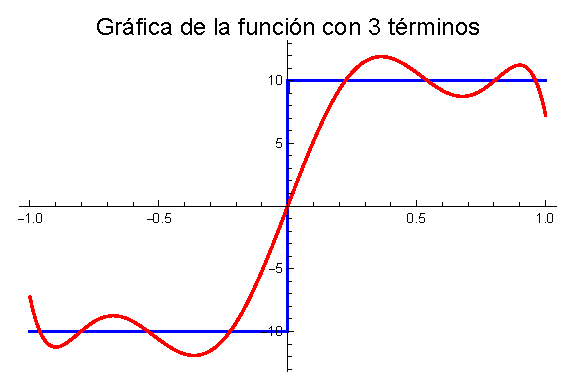
\includegraphics[scale=1]{Imagenes/Expansion_Legendre_V_03.eps}
    \caption{La aproximación para la función $f (x)$ con 3 términos de la serie.}
    \label{fig:figura_plot_01}
\end{figure}
\begin{figure}[H]
    \centering
    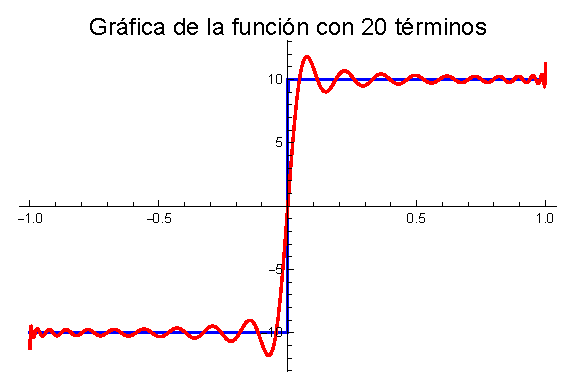
\includegraphics[scale=1]{Imagenes/Expansion_Legendre_V_20.eps}
    \caption{La aproximación para la función $f (x)$ con 20 términos de la serie.}
    \label{fig:figura_plot_02}
\end{figure}
\begin{figure}[H]
    \centering
    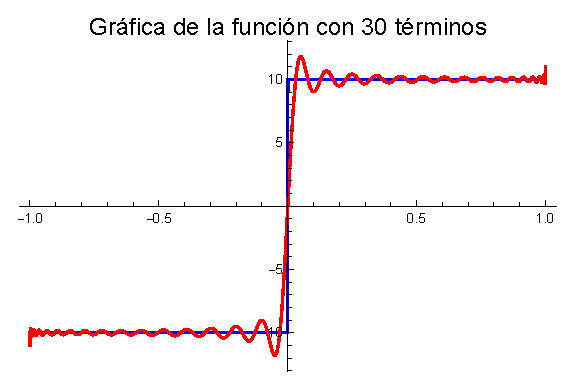
\includegraphics[scale=1]{Imagenes/Expansion_Legendre_V_30.eps}
    \caption{La aproximación para la función $f (x)$ con 30 términos de la serie.}
    \label{fig:figura_plot_03}
\end{figure}
Con la aproximación por series, se reconoce el \textbf{fenómeno de Gibbs} en el punto alrededor de $x = 0$ que es donde cambia de valor la función.

\section{Ecuación radial.}

\subsection{Regresando a la ED.}

En la solución de la ecuación angular, se determina que $\alpha = k (k + 1)$, de esta manera la \textbf{ecuación radial} se escribe como:
\begin{align}
r^{2} \dv[2]{R}{r} + 2 R \dv{R}{r} - k(k + 1) R = 0
\label{eq:ecuacion_26_28}
\end{align}
Como en la ED se tiene que $p_{2} (0) = 0$, se considera una solución a la ecuación radial de la forma:
\begin{align*}
R (r) = r^{s} \nsum_{n=0}^{\infty} b_{n} \, r^{n}
\end{align*}
es decir, hacemos un desarrollo con el método de Frobenius.
\par
La solución general a la ecuación radial es entonces:
\begin{align*}
R_{k} (r) \equiv A_{k} \, r^{k} + \dfrac{B_{k}}{r^{k+1}} \hspace{0.3cm} k = 0, 1, 2, \ldots
\end{align*}
con $A_{k}$ y $B_{k}$ coeficientes por determinar.

\subsection{Solución completa.}

Para encontrar la solución general a la ecuación de Laplace en coordenadas esféricas con una simetría azimutal: multiplicamos la solución radial y angular (dada por los polinomios de Legendre) para cada $k$ y se suma en todos los valores posibles de $k$:
\begin{align}
\psi(r, \theta) = \nsum_{k=0}^{\infty} \left( A_{k} \, r^{k} + \dfrac{B_{k}}{r^{k+1}} \right) \, P_{k} (\cos \theta)
\label{eq:ecuacion_26_29}
\end{align}
donde se ha cambiado $\cos \theta$ por $u$.

\section{Esferas y temperaturas.}
\subsection{Planteamiento.}

Dos hemisferios sólidos conductores de calor de radio $a$, separados por un pequeño espacio aislante, forman una esfera. Las dos mitades de la esfera están en contacto en el exterior, con dos baños de calor (infinitos) a temperaturas $T_{0}$ y $-T_{0}$.
\begin{figure}[H]
    \centering
    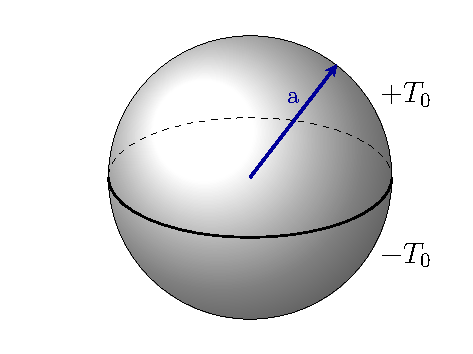
\includegraphics[scale=1.2]{Imagenes/Ejemplo_Esfera_01.eps}
    \caption{Dos hemisferios a distintas temperaturas.}
    \label{fig:figura_esfera_01}
\end{figure}
\textbf{Queremos encontrar la distribución de temperatura $T (r, \theta, \varphi)$ en puntos dentro de la esfera.}
\par
Ya tenemos una expresión que nos permitirá resolver el ejercicio, considerando algunos puntos importantes. En este ejercicio se muestra que es muy importante tomar en cuenta las características que presenta un problema: geometría involucrada, ecuación que modela el fenómeno, técnica de solución a la ecuación, etc.

\subsection{Identificando puntos importantes.}

Elegimos un sistema de coordenadas esféricas en el que el origen coincide con el centro de la esfera y el eje polar es perpendicular al plano ecuatorial.
\par
Suponemos que el hemisferio con temperatura $T_{0}$ es el hemisferio norte, el hemisferio sur está a la temperatura $-T_{0}$.
\par
Dado que el problema tiene simetría azimutal,  $T$ es independiente de $\varphi$, y podemos escribir inmediatamente la solución general con simetría azimutal de la ecuación Laplace en coordenadas esféricas:
\begin{align*}
\psi (r, \theta) = \nsum_{k=0}^{\infty} \left( A_{k} \, r^{k} + \dfrac{B_{k}}{r^{k+1}} \right) \, P_{k} (\cos \theta)
\end{align*}
Sin embargo, dado que el origen $r = 0$ está en la región de interés,  debemos excluir todos los potencias negativas de $r$. Esto se logra haciendo que $B_{k} = 0$.
\par
Así, tenemos que:
\begin{align}
T (r, \theta) = \nsum_{n=0}^{\infty} A_{n} \, r^{n} \, P_{n} (\cos \theta)
\label{eq:ecuacion_26_50}
\end{align}
Quedando pendiente el cálculo de los coeficientes $A_{n}$. Para resolver esta parte, revisemos que:
\begin{align*}
T (a, \theta) = \begin{cases}
T_{0} & \mbox{ si } 0 \leq \theta < \dfrac{\pi}{2} \\[1em]
-T_{0} & \mbox{ si } \dfrac{\pi}{2} < \theta \leq \pi
\end{cases}
\end{align*}
En términos de $u = \cos \theta$, queda expresado por:
\begin{align}
\begin{aligned}
T (a, u) &= \begin{cases}
-T_{0} & \mbox{ si } -1 \leq u < 0 \\[1em]
T_{0} & \mbox{ si } 0 < u \leq 1
\end{cases} = \\[0.5em]
&= \nsum_{n=0}^{\infty} A_{n} \, a_{n} \, P_{n} (u)
\end{aligned}
\label{eq:ecuacion_26_51}
\end{align}
Excepto por el uso de $u$ en lugar de $x$,  es completamente equivalente a la expansión del ejemplo que revisamos. Encontramos que los coeficientes pares están ausentes y:
\begin{align*}
c_{2k+1} \equiv A_{2k+1} \, a^{2k+1} = \dfrac{(-1)^{k} (4 \, k + 3)(2 \, k)!}{2^{2k+1} \, k! \, (k+1)!} \, T_{0}
\end{align*}
Despejando $A_{2k+1}$ de la ecuación anterior, para utilizarlo dentro de la ec. (\ref{eq:ecuacion_26_50})  nos lleva a la solución, que \textbf{determina la temperatura en puntos interiores de la esfera}:

\begin{align}
\begin{aligned}
T (r, \theta) &= T_{0} \, \nsum_{k=0}^{\infty} \dfrac{(-1)^{k} (4 \, k {+} 3)(2 \, k)!}{2^{2k+1} \, k! \, (k {+} 1)!} \, \left( \dfrac{r}{a} \right)^{2k+1} \, P_{2k+1} (\cos \theta)
\end{aligned}
\label{eq:ecuacion_26_52}
\end{align}
donde se ha sustituido $\cos \theta$ por $u$.

\section{Esferas y potenciales.}
\subsection{Entendiendo el ejercicio.}

Considera dos hemisferios eléctricamente conductores de radio $a$ separados por un pequeño espacio aislante en el ecuador. El hemisferio superior se mantiene en el potencial $V_{0}$ y el inferior en $-V_{0}$.
\begin{figure}[H]
    \centering
    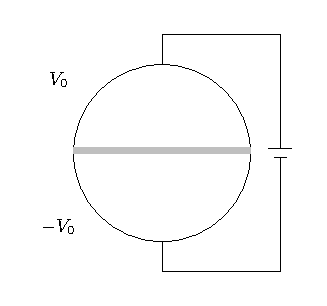
\includegraphics[scale=1]{Imagenes/Ejemplo_Esfera_03.eps}
    \caption{Dos hemisferios conductores cada uno con un potencial. El hemisferio superior tiene un rango para el ángulo polar $0 \leq \theta < \pi/2$ o $0 < \cos \theta \leq 1$, mientras que el hemisferio inferior tiene el rango $\pi/2 < \theta \leq \pi $ o $-1 \leq \cos \theta < 0$.}
    \label{fig_figura_esfera_03}
\end{figure}
\textbf{Queremos encontrar el potencial en puntos fuera de la esfera resultante}.
\par
Dado que el \textbf{potencial debe anularse en el infinito},  esperamos que el primer término en la ecuación (\ref{eq:ecuacion_26_29}) esté ausente,  es decir, debe de ocurrir que $A_{k} = 0$.
\par
Para encontrar $B_{k}$, sustituimos $a$ por $r$ en la ec. (\ref{eq:ecuacion_26_29}), y sea $\cos \theta \equiv u$. Entonces:
\begin{align*}
\psi (a, u) = \nsum_{k=0}^{\infty} \underbrace{\dfrac{B_{k}}{a^{k+1}}}_{\mbox{\large $\equiv c_{k}$}} \, P_{k} (u)
\end{align*}
Donde:
\begin{align*}
\psi (a, u) = \begin{cases}
- V_{0} & \mbox{ si } -1 \leq u < 0 \\[1em]
+ V_{0} & \mbox{ si } 0 < u \leq 1
\end{cases}
\end{align*}
El cálculo de los coeficientes es idéntico al del ejemplo anterior. Por lo tanto, $c_{k} = 0$ para $k$ par, además:
\begin{align*}
c_{2m+1} = \dfrac{B_{2m+1}}{a^{2m+2}} = (-1)^{m} \, \dfrac{(4 m + 3)(2 m)!}{2^{2m+1} (m + 1)! m!} \, V_{0}
\end{align*}
Que despejando para los coeficientes $B_{2m+1}$:
\begin{align*}
B_{2m+1} = \dfrac{(-1)^{m} \, (4 m + 3)(2 m)!}{2^{2m+1} m! (m + 1)!} \, a^{2m+2} \, V_{0}
\end{align*}
Una vez que se calcularon los coeficientes, el potencial queda dado por:
\begin{align}
\begin{aligned}
\psi (r, \theta) &= V_{0} \nsum_{m=0}^{\infty} (-1)^{m} \, \dfrac{(4 m + 3)(2 m)!}{2^{2m+1} m! (m + 1)!} \, \left( \dfrac{a}{r} \right)^{2m+2} \, P_{2m+1} (\cos \theta)
\end{aligned}
\label{eq:ecuacion:26_53}
\end{align}

% \section{Ejercicio esfera aterrizada.}

% Veamos otro ejemplo de la solución de la ecuación de Laplace en coordenadas esféricas, consideremos una esfera conductora neutra puesta a tierra de radio $a$ colocada en un campo eléctrico originalmente uniforme $E_{0}$ que se supone que tiene una extensión infinita, como se muestra en la figura (\ref{fig:figura_esfera_aterrizada})).
% \begin{figure}[H]
%     \centering
%     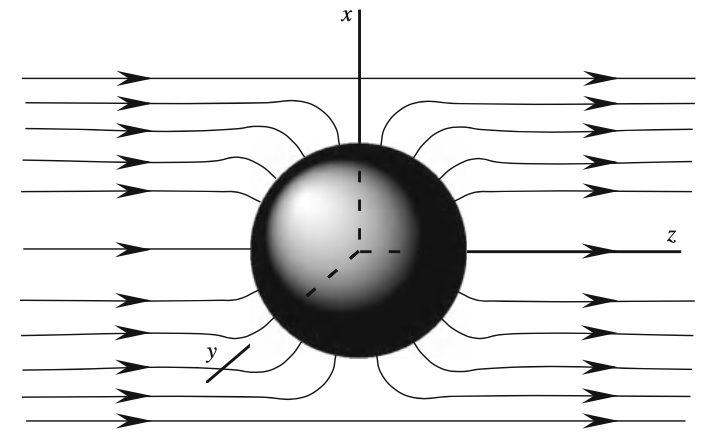
\includegraphics[scale=0.4]{Imagenes/Esfera_Compo_Electrico.png}
%     \caption{El campo eléctrico en la vecindad de una esfera colocada en un campo uniforme externo cambiará, pero el campo alejado de la esfera permanecerá casi uniforme.}
%     \label{fig:figura_esfera_aterrizada}
% \end{figure}

% \textbf{Queremos encontrar el potencial electrostático en todas partes fuera de la esfera}.
% \par
% Eligiendo que el campo esté en la dirección $z$ positiva y colocando el centro de la esfera en el origen, tendremos un problema que presenta simetría azimutal. Por lo tanto, la solución general viene dada por la ec. (\ref{eq:ecuacion_26_29}). Los límites por fuera de la esfera consisten en la esfera misma así como en el infinito. El campo eléctrico en el infinito es el campo uniforme original, porque el campo debido a las cargas inducidas en la esfera desaparece en el infinito. El potencial de este campo (en el infinito) se puede deducir de:
% \begin{align*}
% \vb{E} &= E_{0} \, \vu{e}_{z} = - \grad{\Phi} \\[0.5em]
% \Rightarrow \hspace{0.2cm} E_{0} &= - \pdv{\Phi}{z}, \hspace{1cm} \pdv{\Phi}{x} = \pdv{\Phi}{y} = 0
% \end{align*}
% Por lo tanto, el potencial en el infinito es independiente de $x$ e $y$, y se puede escribir como:
% \begin{align*}
% \Phi (r, \theta) &= - E_{0} \, z = \\[0.5em]
% &= - E_{0} \, r \, \cos \theta = \\[0.5em]
% &= - E_{0} \, r \, P_{1} (\cos \theta) \hspace{1cm} \mbox{para } r \to \infty
% \end{align*}
% Por lo tanto, el potencial en el infinito es independiente de $x$ e $y$, y se puede escribir como:

\section{Ejercicios a cuenta.}
\subsection{Ejercicios.}

\begin{enumerate}
%Ref. Arfken (2006) 12.1.3
\item Demuestra que el potencial electrostático producido por una carga $q$ en $z = a$ para $r < a$ es:
\begin{align*}
\varphi(\vb{r}) = \dfrac{q}{4 \pi \epsilon_{0} a} \, \nsum_{n=0}^{\infty} \left( \dfrac{r}{a} \right)^{n} \, P_{n}(\cos \theta)
\end{align*}
\item Una esfera conductora de calor de radio $a$ está compuesta por dos hemisferios con un espacio infinitesimal aislante entre ellos, como se muestra en la figura (\ref{fig:figura2}).
\begin{figure}[H]
    \centering
   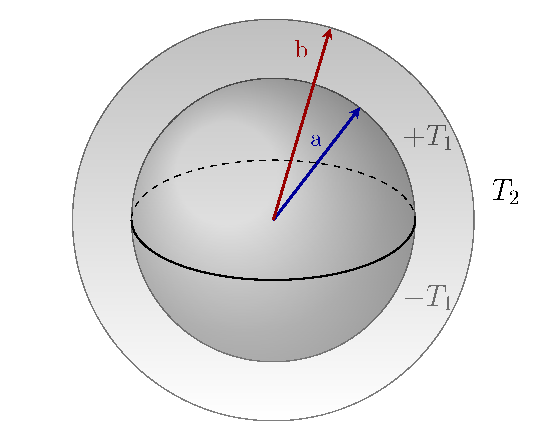
\includegraphics[scale=0.9]{Imagenes/esfera1.eps}
    \caption{Los hemisferios de la esfera interior se encuentran a diferentes temperatura.}
    \label{fig:figura2}
\end{figure}
Las mitades superior e inferior de la esfera están en contacto con baños térmicos de temperaturas $+ T_{1}$ y $-T_{1}$, respectivamente. La esfera de radio $a$ está dentro de otra esfera conductora de calor de radio $b$ con una temperatura $T_{2}$.
\par
Calcula la temperatura:
\begin{enumerate}
\item Dentro de la esfera interior,
\item En la región entre las dos esferas, y
\item Por fuera de la esfera exterior.
\end{enumerate}
%Ref. Boas (20059 Chapter 12. Problems 10, 12)
\item Expande en términos de una serie con Polinomios de Legendre los siguientes polinomios:
\begin{enumerate}
\item $3 \, x^{2} + x - 1$
\item $x - x^{3}$
\end{enumerate}
\end{enumerate}


\end{document}